\documentclass[a4paper,12pt,oneside,openany,table,xcdraw]{article}

\usepackage{setspace}
\usepackage{multirow}
\usepackage{hyperref}
\usepackage{caption}
\usepackage{indentfirst}

\usepackage[brazilian]{babel}
\usepackage[utf8x]{inputenc}
\usepackage{amsmath, graphicx, subfig, enumerate}
\usepackage{float, verbatim}
\usepackage[colorinlistoftodos]{todonotes}
\usepackage{makeidx} % Para o sumário
\usepackage{geometry}

\graphicspath{{img/}}
\geometry{a4paper, hmargin={3cm, 3cm}, vmargin={3cm, 2cm} }
\setlength{\parindent}{1.0cm}
\captionsetup{font=small}

\begin{document}
\newcommand{\thedepartment}{Faculdade de Engenharia Elétrica}
\newcommand{\thecourse}{FEELT}
\newcommand{\thetitle}{CIRCUITOS TRIFÁSICOS DESEQUILIBRADOS}
\newcommand{\thetype}{Relatório da Disciplina de Experimental de Circuitos Elétricos II}
\newcommand{\theproftitle}{Bacharel em Engenharia Elétrica}
\newcommand{\thestudent}{Lesly Viviane Montúfar Berrios\\
\centering11811ETE001}
\newcommand{\theadvisor}{Prof. Wellington Maycon Santos Bernardes}
\newcommand{\thecity}{Uberlândia}

\thispagestyle{empty}\newcommand*{\themonth}{\ifthenelse{\the\month < 2}{Janeiro }
                  {\ifthenelse{\the\month < 3}{Fevereiro }
                  {\ifthenelse{\the\month < 4}{Março }
                  {\ifthenelse{\the\month < 5}{Abril }
                  {\ifthenelse{\the\month < 6}{Maio }
                  {\ifthenelse{\the\month < 7}{Junho }
                  {\ifthenelse{\the\month < 8}{Julho }
                  {\ifthenelse{\the\month < 9}{Agosto }
                  {\ifthenelse{\the\month < 10}{Setembro }
                  {\ifthenelse{\the\month < 11}{Outubro }
                  {\ifthenelse{\the\month < 12}{Novembro }{Dezembro }}}}}}}}}}}}
                  
\begin{titlepage}
\begin{center}

	\vspace{-0.5cm}

  \begin{figure}[hbt!]
		\begin{center}
		   
\includegraphics[width=2.8cm]{ufu-logo.png}
		\end{center}
	\end{figure}
 	%\vspace{-4cm}

%\begin{doublespacing}

  \Large{\textbf{Universidade Federal de Uberlândia}}\\
  \large{\thedepartment}\\
  \large{\thecourse}\\


\vspace{5.8cm}
  \par
  \large\textbf{\thetitle}
\vspace{5.8cm} 

%\end{doublespacing}
  \par
  \thetype\\
  por\\
  %\hspace{2cm}\large{}\\

\vspace{0.8cm}
\par
  \normalsize{\thestudent}\\ [2cm]
  \theadvisor

\par\vfill
  \thecity, \themonth / \the\year

\end{center}

\end{titlepage}

%% Comeca o documento !

\onehalfspacing
\tableofcontents % sumário
\newpage

\section{Objetivos} % 2,5%


\section{Introdução teórica} % 5%


\section{Preparação}
\subsection{Materiais e ferramentas} % 2,5%
\begin{enumerate}[1 -]
\item \emph{\textbf{Fonte:}}
Alimentará todo o circuito. Possui frequência de $60Hz$.

\item \emph{\textbf{Regulador de tensão (Varivolt):}}
Também chamado de autotransformador, permitirá obter o valor desejado de corrente a partir da regulagem correta da tensão fornecida pela fonte.

\item \emph{\textbf{Conectores:}}
Para as conexões no circuito foi utilizado majoritariamente cabos banana-banana.

\item \emph{\textbf{Medidor eletrônico KRON Mult K:}}
Possibilita encontrar a medição da potência real (P) - vatímetro, reativa (Q) e aparente (S) do circuito. Ele também possui função de cofasímetro, instrumento elétrico que mede o fator de potência (fp, $cos\theta$) ou o ângulo da impedância $\theta$ do circuito, para um circuito com a impedância $Z = Z\angle \theta$.

\item \emph{\textbf{Amperímetro analógico AC:}}
Instrumento utilizado para acompanhar visualmente o aumento da corrente.

\item \emph{\textbf{Reatores de 200 mH:}}
Foram utilizados 3, para compor a carga do circuito trifásico. Sendo $L=160mH$ e $R_L=3,8\Omega$.

\item \emph{\textbf{Resistores de $50\Omega$:}}
Foram utilizados 3, para compor a carga do circuito trifásico.

\item \emph{\textbf{Capacitores de $45,9\mu F$:}}
Foram utilizados 3, para compor a carga do circuito trifásico. Sendo $C= 45,9\mu F$. %%%%%%%%%%%Resistencia dos capacitores? 

\end{enumerate}

\subsection{Montagem} % 2,5%

\subsection{Carga em estrela com neutro conectado}
A montagem utilizada observa-se na Figura \ref{m1:esquema}. Pretende-se com este circuito investigar-se acerca do efeito do neutro em circuitos trifásicos desequilibrados. Usou-se TL=0000, TC=TP=1 como configurações no medidor \emph{Kron}.
\begin{figure}[H]
\centering
\captionsetup{font=scriptsize}
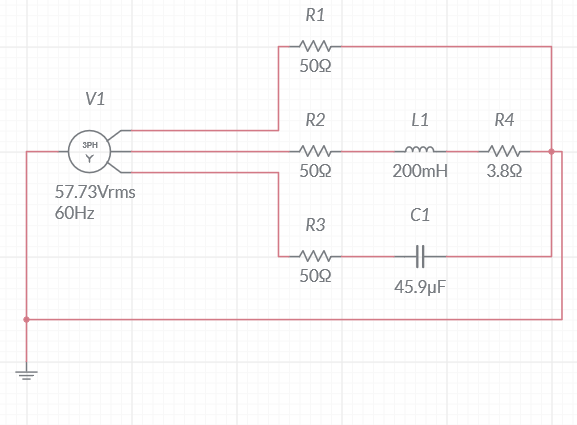
\includegraphics[width=14cm]{m1-esquema}
\caption{Circuito esquemático da montagem 1.}
\label{m1:esquema}
\end{figure}
Observa-se que a tensão de linha rms utilizada é de $100V$, no entanto para a simulação com neutro conectado deve-se usar gerador conectado em estrela que entregará uma tensão de fase $V_F=57,73$

\section{Dados Experimentais}

\subsection{Carga em estrela com neutro conectado}

\begin{table}[H]
\centering
\caption{Dados experimentais referentes à primeira montagem: carga em estrela com neutro conectado.}
\label{m1:dados:abc}
\resizebox{\textwidth}{!}{%
\begin{tabular}{c|c|c|c|c|c|c|c|c|c|}
\cline{2-10}
                        & $V_L$ (V) & $V_F$ (V) & $I_L$ (A) & P (W) & Q (VAr) & S (VA) & fp    & $A_N$ (A)             & $V_{N'N}$  (V)        \\ \hline
\multicolumn{1}{|c|}{A} & 96,10     & 55,89     & 1,13      & 63,84 & 0,30    & 64,16  & 1     & \multirow{3}{*}{0,21} & \multirow{3}{*}{0} \\ \cline{1-8}
\multicolumn{1}{|c|}{B} & 10,07     & 56,57     & 0,62      & 22,12 & 27,68   & 35,58  & 0,625 &                       &                    \\ \cline{1-8}
\multicolumn{1}{|c|}{C} & 99,69     & 58,82     & 0,76      & 29,54 & 33,44   & 44,50  & 0,659 &                       &                    \\ \hline
\end{tabular}%
}
\end{table}

\section{Análise teórica do circuito}


\section{Análise sobre segurança} % 2,5%
Os óculos de segurança são Equipamentos de Proteção Individual (EPIs) e são utilizados para a proteção da área ao redor dos olhos contra qualquer tipo de detrito estranho, que possa causar irritação ou ferimentos. Também protegem contra faíscas, respingos de produtos químicos, detritos, poeira, radiação e etc \cite{safe}.
É importante a utilização desse equipamento durante os experimentos a fim de evitar qualquer dano, além de preparar o profissional para o manejo correto e seguro de qualquer equipamento.
Além disso, foi de extrema importância a presença do professor ou técnico na verificação da montagem do circuito antes de energizá-lo. Assim, reduziu-se riscos de curtos-circuitos ou sobrecarga na rede.


\section{Cálculos, análise dos resultados e questões} % (quando houver) (70%)


\newpage
\section{Simulação computacional} % (10%);



\section{Conclusões} % (no mínimo 10 linhas) (5%);


\newpage
\begin{thebibliography}{9} 
% Introdução
\bibitem{ph}
    P. H. O. Rezende,
    "Circuitos Polifásicos Equilibrados", 2018.

\bibitem{irwin}
    J. D. Irwin,
    “Análise de Circuitos Em Engenharia”, Pearson, $4^a$ Ed., 2000.

\bibitem{boylestad}
    R. L. Boylestad,
    “Introdução À Análise de Circuitos”, Pearson, $10^a$ Ed., 2004.

\bibitem{safe}
    SafetyTrabi,
    “Óculos de segurança: Saiba quando utilizar este EPI”, SafetyTrab, 2019.
 Disponível em:
 \url{https://www.safetytrab.com.br/blog/oculos-de-seguranca/}. Acesso em: ago. 2019.


\end{thebibliography}
\end{document}
